\documentclass[12pt]{article}
\linespread{1.2}
\usepackage[margin=2cm]{geometry}
\usepackage[utf8]{inputenc}
\usepackage{amsfonts}
\usepackage{amsmath}
\usepackage{multicol}
\usepackage{amsthm}
\usepackage{amssymb,scrextend}
\usepackage{graphicx,tikz}
\newtheorem{dfn}{Definition}
\renewcommand{\qed}{\hfill$\blacksquare$}
\let\newproof\proof
\renewenvironment{proof}{\vspace{1em}\begin{addmargin}[2em]{0em}\begin{newproof}}{\end{newproof}\end{addmargin}\qed}
\newenvironment{theorem}[2][Theorem]{\begin{trivlist}
\item[\hskip \labelsep {\bfseries #1} \hskip \labelsep {\bfseries #2.}]}{\end{trivlist}}
\newenvironment{example}[2][Example]{\begin{trivlist}
\item[\hskip \labelsep {\bfseries #1} \hskip \labelsep {\bfseries #2.}]}{\end{trivlist}}
\newenvironment{lemma}[2][Lemma]{\begin{trivlist}
\item[\hskip \labelsep {\bfseries #1} \hskip \labelsep {\bfseries #2.}]}{\end{trivlist}}
\newenvironment{exercise}[2][Exercise]{\begin{trivlist}
\item[\hskip \labelsep {\bfseries #1} \hskip \labelsep {\bfseries #2.}]}{\end{trivlist}}
\newenvironment{problem}[2][Problem]{\begin{trivlist}
\item[\hskip \labelsep {\bfseries #1} \hskip \labelsep {\bfseries #2.}]}{\end{trivlist}}
\newenvironment{corollary}[2][Corollary]{\begin{trivlist}
\item[\hskip \labelsep {\bfseries #1} \hskip \labelsep {\bfseries #2.}]}{\end{trivlist}}
\usepackage{fancyhdr,enumitem,changepage,url}
\pagestyle{fancy}
\author{Warren Atkison}
\date{\today}
\setlength{\headheight}{15pt}
\begin{document}
\fancyhf{}
\fancyhead[L]{Warren Atkison}
\fancyhead[C]{Homework Set 7}
\fancyhead[R]{\today}
\fancyfoot[R]{\thepage}

\begin{exercise}{5.7.3 (2pt)}
	Suppose $G$ is simple with degree sequence $d_1 \le d_2 \le \ldots \le d_n$, and for $k \le n - d_n - 1$, $d_k \ge k$. Show $G$ is connected
\end{exercise}

\begin{proof}
	Suppose $G$ is not connected. Consider a connected subgraph of $G$ containing $v_n$ and all its neighbors, which has $d_n + 1$ vertices. Now Consider another connected subgraph of $G$, $G'$ not connected to $v_n$ with $m$ vertices, then $m \le n - (d_n + 1)$ so $d_m \ge m$. Let the largest degree of our subgraph with $m$ vertices be $d_i$, so $d_i \le m - 1$. However then
	\[
		m \le d_m \le d_i \le m - 1
	\]
	and we have a contradiction.
\end{proof}
\begin{exercise}{5.7.4 (2pt)}
	Recall that a graph is $k$-regular if all the vertices have degree $k$. What is the smallest integer $k$ that makes this true:
	\begin{enumerate}
		\item[] If $G$ is simple, has $n$ vertices, $m \ge k$, and $G$ is $m$-regular, then $G$ is connected.
	\end{enumerate}
\end{exercise}	
If $n$ is even, then the smallest $k$ is $n/2$. If $n$ is odd, then the smallest $k$ is $(n-1)/2$. This is because any less and we can split $G$ into 2 graphs of $K_{n/2}$ if $n$ is odd, and $K_{(n+1)/2} + K_{(n-1)/2}$ if $n$ is even, which has is $n/2 - 1$ regular in the even case and $(n-1)/2 - 1$ regular in the odd case.
\begin{exercise}{5.7.5 (2pt)}
	Suppose $G$ has at least one edge. Show that $G$ is 2-connected if and only if for all vertices $v$ and edges $e$ there is a cycle containing $v$ and $e$.
\end{exercise}	
\begin{proof}
	Let $G$ be 2-connected. Suppose there is no cycle containing $v$ and $e$. Then, $v$ and $e$ must be connected by a path otherwisee containing a bridge, otherwise $v$ and $e$ would not be connected or $v$ and $e$ would form a cycle. However, since the path contains a bridge, then $G$ is not 2 connected and we have a contradiction.

	For all vertices $v$ and $e$ in a graph $G$, let there be a cycle containing $v$ and $e$. Then in order to disconnect any 2 vertices we would need to remove at least 2 vertices, one for either direction along the cycle, so $G$ is 2-connected.
\end{proof}
\begin{exercise}{5.7.6 (2pt)}
	Find a simple graph with $\kappa(G) < \lambda(G) < \delta(G)$.
\end{exercise}	
Consider the following graph $G$:
\begin{center}
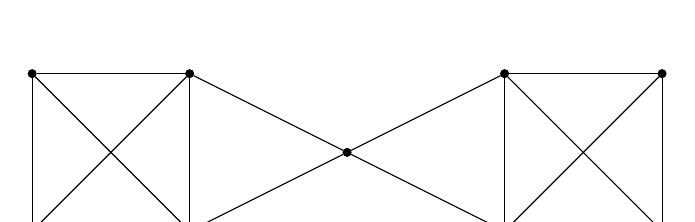
\begin{tikzpicture}[scale=2]
  % Nodes
  \foreach \i/\x/\y in {0/0/0, 1/1/0, 2/1/1, 3/0/1}{
    \node[draw, circle, fill=black, inner sep=1pt] (v\i) at (\x,\y) {};
  }
  % Edges
  \foreach \i in {0,1,2,3}{
    \foreach \j in {\i,...,3}{
      \ifnum\i=\j\relax\else
        \draw (v\i) -- (v\j);
      \fi
    }
  }
  
  \foreach \i/\x/\y in {4/3/0, 5/4/0, 6/4/1, 7/3/1}{
    \node[draw, circle, fill=black, inner sep=1pt] (v\i) at (\x,\y) {};
  }
  % Edges
  \foreach \i in {4,5,6,7}{
    \foreach \j in {\i,...,7}{
      \ifnum\i=\j\relax\else
        \draw (v\i) -- (v\j);
      \fi
    }
  }

  \node[draw, circle, fill=black, inner sep=1pt] (v8) at (2,0.5) {};
	
  \foreach \i in {1,2,4,7}{
	  \draw (v\i) -- (v8);
  }

\end{tikzpicture}
\end{center}
\[
	\kappa(G) = 1 < \lambda(G) = 2 < \delta(G) = 3
\]
\begin{exercise}{5.4.2 (2pt)}
	What is the smallest number of edges that can be removed from $K_5$ to create a bipartite graph?
\end{exercise}	
We can turn $K_5$ into $K_{2,3}$ by removing the four red edges:
\begin{center}
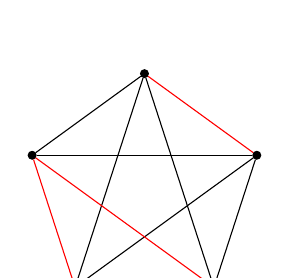
\begin{tikzpicture}
  % Nodes
  \foreach \i in {0,1,2,3,4}{
    \node[draw, circle, fill=black, inner sep=1pt] (v\i) at ({360/5 * \i + 18}:1.5cm) {};
  }
  % Edges
  \draw (v0) -- (v1) [red];
  \draw (v2) -- (v3) [red];
  \draw (v3) -- (v4) [red];
  \draw (v1) -- (v2);
  \draw (v4) -- (v0);
  \draw (v0) -- (v2);
  \draw (v0) -- (v3);
  \draw (v1) -- (v3);
  \draw (v1) -- (v4);
  \draw (v2) -- (v4) [red];
\end{tikzpicture}
\end{center}
This is the smallest number of edges we can remove since $K_{2,3}$ has 6 total edges and our only other option $K_{1,4}$ has only 4 edges, so we'd have to remove more edges.
\begin{exercise}{5.5.1 (2pt)}
	Suppose that $G$ is a connected graph, and that every spannig tree contains edge $e$. Show that $e$ is a bridge.
\end{exercise}	
\begin{proof}
	Suppose $e$ is not a bridge. Then $G - {e}$ is a connected graph, and it has a spanning tree. However, this spanning tree would also be a spanning tree of $G$ which does not contain $e$, so we have a contradiction.
\end{proof}
\end{document}
